\subsection*{Database}
Systemet skal som nævnt i kravspecifikationer have forbindelse til en database. Denne kan tilgås fra den tilhørende controller. Klasserne for databasen og controlleren fremgår af \autoref{fig:MVCDatabase}. 

\begin{figure} [H]
\centering
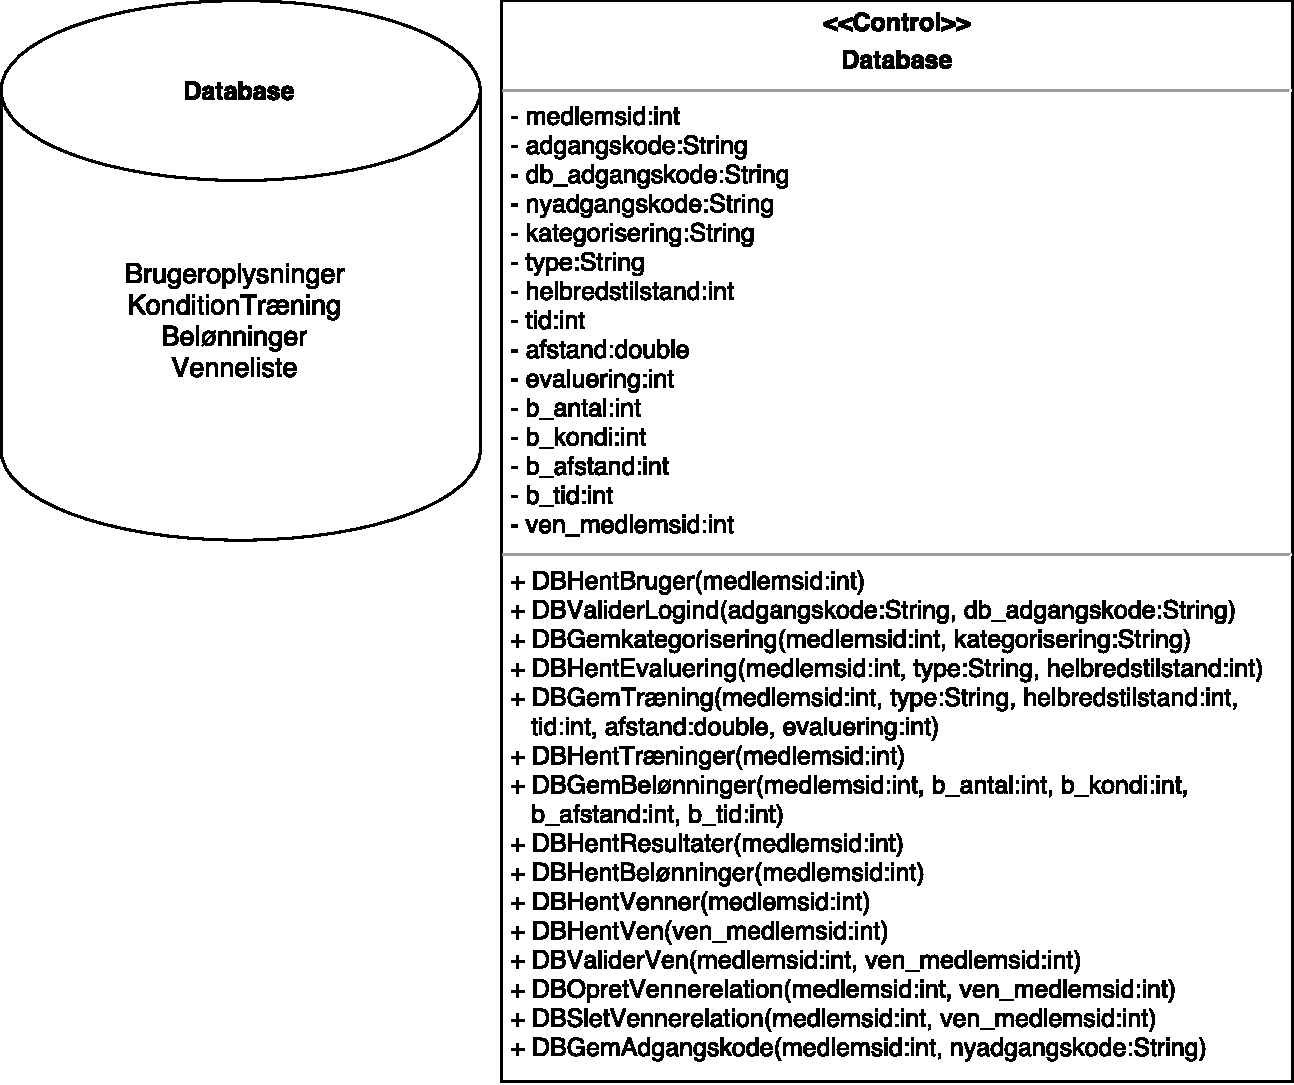
\includegraphics[width=0.5\textwidth]{figures/MVC/MVCDatabase}
\caption{Designklasser for Database. Til venstre ses databasen og til højre ses den tilhørende controller.}
\label{fig:MVCDatabase}
\end{figure}

\noindent
Databasen indeholder Brugeroplysninger, Venneliste og KonditionResultater. Brugeroplysninger indeholder alle brugerens oplysninger. Disse registreres i forbindelse med rehabiliteringsforløbet af sundhedspersonalet, som senere kan tilgå disse og redigere i brugeroplysningerne. Vennelisten indeholder andre bruger som brugeren følger, derudover har brugeren mulighed for at tilføje flere brugere til sin venneliste. KonditionResultater har brugerens resultater for konditionstræning. Sundhedspersonalet og brugeren har mulighed for at tilgå denne. 

Designet af databasen er beskrevet i et ER-diagram og vil fremgå af \autoref{sec:ER}. \textit{Database} controlleren indeholder metoderne Gem, Send og Modtag. Disse har til formål at kommunikere mellem databasen og de forskellige controllere. Der oprettes forbindelse til denne ved log ind, hvor Brugeroplysninger, Venneliste og KonditionResultater sendes og gemmes i forskellige entitys.

\subsection*{Lagring af data}  \label{sec:entity}
Når der oprettes forbindelse til databasen ved log ind, sendes og gemmes data i tre forskellige entity, som fremgår af \autoref{fig:MVCEntity}. Der er valgt at udarbejde entitys for ikke at skulle tilgå databasen hver gang data skal hentes. Dertil er det også muligt at opdele data, som har med en specifik controller at gøre, så irrelevant data undgås. 

\begin{figure} [H]
\centering
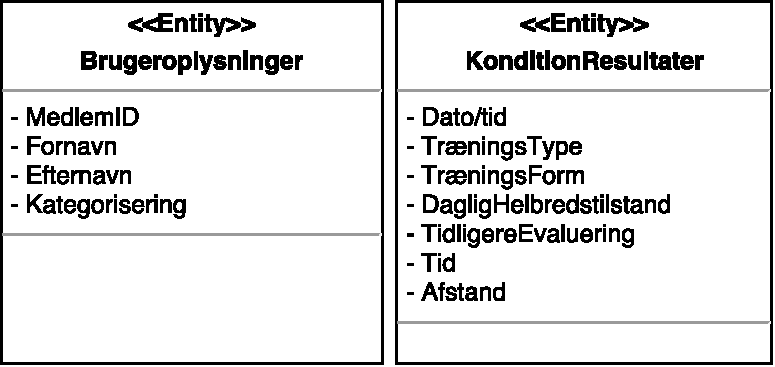
\includegraphics[width=0.9\textwidth]{figures/MVC/Entity}
\caption{Designklasser for Entitys, herunder Brugeroplysninger, Vennelsite og KonditionResultater. Attributterne er markeret med \#, hvilket indikerer, at disse er beskyttede.\fxnote{Skal alle være beskyttede??}}
\label{fig:MVCEntity}
\end{figure}

\noindent
På \autoref{fig:MVCEntity} fremgår det, at de forskellige attributter er beskyttede. Dette er gjort, da det ønskes at attributterne kun kan tilgås indenfor det samme projekt. 
\textit{Brugeroplysninger} indeholder informationer om brugeren, herunder MedlemsID, Adgangskode, Fornavn, Efternavn og Kategorisering. 
\textit{Venneliste} har informationer om andre brugere, der følges, såsom VenMedlemsID, VenFornavn, VenEfternavn og VenBelønninger. 
\textit{Resultater} indeholder brugerens resultater, som er defineret ud fra DatoTid, TræningsType, TræningsForm, DagligHelbredstilstand, Evaluering, Tid, Afstand, KompatibleMåleenheder og Belønninger. 
